\documentclass[11pt,a4paper]{article}
\usepackage[margin=2cm]{geometry}
\usepackage{amsmath,amssymb,booktabs,array,graphicx,caption,needspace}
\usepackage[T1]{fontenc}
\usepackage[hidelinks]{hyperref}
\captionsetup{font=small,labelfont=bf,width=0.95\linewidth}
\graphicspath{{../../results/figures/}}
\setlength{\tabcolsep}{3.5pt}
\title{Controlled turbulence-sensitivity study:\\ error of the analytic averages versus $\sigma_X^2$ at fixed distance}
\author{Computed from the repository \texttt{tfqkd-fso-turbulence}}
\date{22 October 2026}
\begin{document}\maketitle

\section{Design of the study}
\paragraph{What is varied.} For each fixed total distance $L\in\{80,120,160\}$~km the variance of the log-transmittance $X=\ln(\eta/\eta_0)$, $\eta=\sqrt{\eta_A\eta_B}$, is imposed on a grid $\sigma_X^2\in\{0.005,0.01,0.02,0.05,0.1,0.2,0.3,0.4,0.5,0.6,0.7,0.8\}$, independently of $L$. \textbf{This is a controlled sensitivity study.} The imposed $\sigma_X^2$ values are not claimed to correspond to atmospheric conditions realisable at that distance; the distance enters only through the deterministic transmittance $\eta_0=\sqrt{\eta_{\rm FSO}(L)}$ ($0.0393,\ 0.00757,\ 0.00175$ at $80,120,160$~km, i.e.\ the operating point on the key-rate curve). Where the channel model does tie $\sigma_X^2$ to the atmosphere this is stated below.

\paragraph{Three channel models.}
\begin{itemize}
\item \textbf{LN}: $X\sim\mathcal N(-\sigma_X^2,\sigma_X^2)$ (manuscript model; $\sigma_X^2=\sigma_R^2(L/2)/2$ per arm pair).
\item \textbf{GG}: independent Gamma--Gamma arms, $X=\tfrac12(\ln I_A+\ln I_B)$, $\mathrm{Var}(X)=c_2=\tfrac12[\psi'(\alpha)+\psi'(\beta)]$ with $(\alpha,\beta)$ from the plane-wave Andrews--Phillips formulas (exponent $6/5$ on the Rytov variance, as in the repository code). For each target $\sigma_X^2$ the per-arm Rytov variance is solved from $c_2(\sigma_R^2)=\sigma_X^2$ on the rising branch. \emph{$c_2$ is bounded:} its maximum over all $\sigma_R^2$ is $0.858$ (at $\sigma_R^2\approx52$), because Gamma--Gamma saturates; this fixes the upper end of the grid. The grid values $\ge$ about $0.85$ would correspond to saturated moderate/strong turbulence.
\item \textbf{GG+BB}: as GG, with turbulence-induced long-term beam broadening (which contains beam wander) per arm, $\eta_0\to\eta_0f_{\rm bb}$, $W_{\rm LT}^2=W^2(1+1.63\,\sigma_R^{12/5}\Lambda)$, using the $\sigma_R^2$ solved for GG. Broadening therefore changes the operating point, not the fading statistics. In this study $\sigma_R^2$ and $L$ are independent, so $f_{\rm bb}^2$ is that of an arm of length $L/2$ with the imposed $\sigma_R^2$ (listed in the tables); in a real atmosphere both follow from $C_n^2$.
\end{itemize}
\paragraph{Approximations compared} (all with the repository's analytic derivatives, Appendices A--H of the manuscript): \emph{conventional/mean} $\mathbb E[Q]\simeq Q(\bar\eta)+\tfrac12Q''(\bar\eta)\mathrm{Var}(\eta)$ with $\bar\eta=\mathbb E[\eta]$, $\mathrm{Var}(\eta)=\eta_0^2(1-m_1^2)$, $m_1=\mathbb E[e^X]$; \emph{2nd-order median} $Q(\eta_m)+\tfrac{c_2}{2}\Theta^2Q$; \emph{4th-order median} $Q(\eta_m)+\tfrac{c_2}{2}\Theta^2Q+\tfrac{c_3}{6}\Theta^3Q+\tfrac{c_4+3c_2^2}{24}\Theta^4Q$, all at $\eta_m=\eta_0e^{c_1}$ (cumulants $c_n=2^{1-n}\kappa_n$ for GG, $(-\sigma_X^2,\sigma_X^2,0,0)$ for LN).

\paragraph{References (independent of the formulas).} LN: Simpson quadrature in $X$ over $\mu\pm12\sigma$ (40001 points). GG: numerical convolution of the two arms' Bessel-$K$ log-densities (6001 points each; density norm $=1\pm5\times10^{-10}$ in every case). The transmittance is capped at $1$ in the references; the probability of $\eta>1$ is at most $3.2\times10^{-6}$ in all cases, so the cap does not affect the comparison. Errors are $100(\text{approx}-\text{ref})/\text{ref}$.

\paragraph{Where this study touches realistic conditions.} For the weak class $C_n^2=10^{-17}$ the actual values at $L=80,120,160$~km are $\sigma_X^2=0.086,\,0.181,\,0.307$ (LN, manuscript Table) and $c_2=0.084,\,0.166,\,0.258$ (GG). For the moderate class the Gamma--Gamma channel is saturated, $c_2=0.84$--$0.86$ at all three distances (top of the grid), whereas the log-normal model would give $\sigma_X^2=8.6$--$31$, far outside the tested range. LN results above $\sigma_X^2=0.8$ were not computed.

\section{Turbulence-sensitivity tables}
Tables~\ref{tab:sens-LN}--\ref{tab:sens-GGBB} give all $3\times3\times12$ cases. Table~\ref{tab:thr} condenses the key rate; Table~\ref{tab:thr2} the maximum errors of $e_X$ and $e_Z$.

\begin{table}[htbp]\centering\small
\caption{Secret key rate $R$: $\sigma_X^2$ at which $|{\rm error}|$ first exceeds $0.1\%$ / $1\%$ (log-linear interpolation on the grid; $>0.8$ = not reached within the grid), and the maximum $|{\rm error}|$ [\%] over $0.005\le\sigma_X^2\le0.8$.}
\label{tab:thr}
\begin{tabular}{llccc}\toprule
model & $L$ [km] & mean: $0.1\%$ / $1\%$ / max & 2nd: $0.1\%$ / $1\%$ / max & 4th: $0.1\%$ / $1\%$ / max\\\midrule
LN & 80 & 0.54 / $>0.8$ / 0.26 & 0.08 / 0.25 / 8.15 & 0.28 / 0.65 / 1.72 \\
LN & 120 & 0.34 / $>0.8$ / 0.76 & 0.09 / 0.28 / 7.21 & 0.34 / 0.78 / 1.07 \\
LN & 160 & 0.22 / 0.62 / 1.87 & 0.08 / 0.27 / 8.03 & 0.35 / 0.78 / 1.09 \\
\midrule
GG & 80 & $>0.8$ / $>0.8$ / 0.04 & 0.12 / 0.46 / 1.40 & 0.36 / 0.69 / 1.74 \\
GG & 120 & 0.59 / $>0.8$ / 0.13 & 0.15 / $>0.8$ / 0.90 & 0.36 / 0.70 / 1.65 \\
GG & 160 & 0.34 / $>0.8$ / 0.29 & 0.15 / $>0.8$ / 0.96 & 0.34 / 0.68 / 1.83 \\
\midrule
GG+BB & 80 & 0.79 / $>0.8$ / 0.10 & 0.13 / 0.51 / 1.12 & 0.36 / 0.70 / 1.64 \\
GG+BB & 120 & 0.53 / $>0.8$ / 0.23 & 0.15 / $>0.8$ / 0.88 & 0.36 / 0.70 / 1.74 \\
GG+BB & 160 & 0.33 / $>0.8$ / 0.34 & 0.15 / 0.60 / 1.14 & 0.34 / 0.67 / 1.93 \\
\bottomrule\end{tabular}\end{table}

\begin{table}[htbp]\centering\small
\caption{Maximum $|{\rm error}|$ [\%] of $e_X$ and $e_Z$ over $0.005\le\sigma_X^2\le0.8$.}
\label{tab:thr2}
\begin{tabular}{llcccccc}\toprule
 & & \multicolumn{3}{c}{$e_X$} & \multicolumn{3}{c}{$e_Z$}\\\cmidrule(lr){3-5}\cmidrule(lr){6-8}
model & $L$ [km] & mean & 2nd & 4th & mean & 2nd & 4th\\\midrule
LN & 80 & 0.000 & 0.025 & 0.003 & 0.521 & 0.065 & 0.011 \\
LN & 120 & 0.004 & 0.154 & 0.019 & 1.078 & 0.084 & 0.004 \\
LN & 160 & 0.060 & 0.580 & 0.059 & 1.964 & 0.230 & 0.010 \\
\midrule
GG & 80 & 0.128 & 0.073 & 0.025 & 0.330 & 0.106 & 0.044 \\
GG & 120 & 0.637 & 0.360 & 0.111 & 0.777 & 0.284 & 0.048 \\
GG & 160 & 2.420 & 1.317 & 0.338 & 1.625 & 0.602 & 0.058 \\
\midrule
GG+BB & 80 & 0.423 & 0.240 & 0.076 & 0.622 & 0.223 & 0.041 \\
GG+BB & 120 & 1.625 & 0.899 & 0.251 & 1.304 & 0.487 & 0.063 \\
GG+BB & 160 & 4.680 & 2.413 & 0.453 & 2.300 & 0.772 & 0.059 \\
\bottomrule\end{tabular}\end{table}

\begin{table}[htbp]
\centering\scriptsize
\caption{Turbulence-sensitivity table, Log-normal. Relative error [\%] of the turbulence-averaged $e_X$, $e_Z$, $R$ for the conventional mean-transmittance (delta) approximation, the 2nd-order and the 4th-order median formula, against the independent quadrature reference, at fixed $L$ and imposed $\sigma_X^2$. $\sigma_R^2$: per-arm Rytov variance implied by $\sigma_X^2=\sigma_R^2/2$ (manuscript convention), not an independent input.}
\label{tab:sens-LN}
\begin{tabular}{rrrrrrrrrrrrr}
\toprule
 & & & & \multicolumn{3}{c}{$e_X$} & \multicolumn{3}{c}{$e_Z$} & \multicolumn{3}{c}{$R$}\\
\cmidrule(lr){5-7}\cmidrule(lr){8-10}\cmidrule(lr){11-13}
$L$ [km] & $\sigma_X^2$ & $\sigma_R^2$ & $f_{\rm bb}^2$ & mean & 2nd & 4th & mean & 2nd & 4th & mean & 2nd & 4th\\
\midrule
80 & 0.005 & 0.01 & -- & $0$ & $0$ & $0$ & $0$ & $0$ & $0$ & $0$ & $-0.0005$ & $0$ \\
 & 0.01 & 0.02 & -- & $0$ & $0$ & $0$ & $0$ & $0$ & $0$ & $0$ & $-0.0018$ & $0$ \\
 & 0.02 & 0.04 & -- & $0$ & $0$ & $0$ & $+0.0002$ & $+0.0001$ & $0$ & $+0.0001$ & $-0.0072$ & $0$ \\
 & 0.05 & 0.1 & -- & $0$ & $0$ & $0$ & $+0.0012$ & $+0.0007$ & $0$ & $+0.0007$ & $-0.045$ & $-0.0007$ \\
 & 0.1 & 0.2 & -- & $0$ & $0$ & $0$ & $+0.0051$ & $+0.0026$ & $0$ & $+0.0027$ & $-0.174$ & $-0.0055$ \\
 & 0.2 & 0.4 & -- & $0$ & $-0.0003$ & $0$ & $+0.022$ & $+0.0093$ & $+0.0003$ & $+0.011$ & $-0.664$ & $-0.041$ \\
 & 0.3 & 0.6 & -- & $0$ & $-0.0011$ & $-0.0001$ & $+0.052$ & $+0.019$ & $+0.0010$ & $+0.027$ & $-1.42$ & $-0.128$ \\
 & 0.4 & 0.8 & -- & $0$ & $-0.0028$ & $-0.0002$ & $+0.099$ & $+0.029$ & $+0.0022$ & $+0.051$ & $-2.42$ & $-0.283$ \\
 & 0.5 & 1 & -- & $0$ & $-0.0055$ & $-0.0004$ & $+0.166$ & $+0.040$ & $+0.0038$ & $+0.084$ & $-3.62$ & $-0.515$ \\
 & 0.6 & 1.2 & -- & $0$ & $-0.0098$ & $-0.0010$ & $+0.255$ & $+0.051$ & $+0.0059$ & $+0.129$ & $-4.99$ & $-0.830$ \\
 & 0.7 & 1.4 & -- & $+0.0001$ & $-0.016$ & $-0.0018$ & $+0.372$ & $+0.059$ & $+0.0084$ & $+0.187$ & $-6.51$ & $-1.23$ \\
 & 0.8 & 1.6 & -- & $+0.0001$ & $-0.025$ & $-0.0032$ & $+0.521$ & $+0.065$ & $+0.011$ & $+0.263$ & $-8.15$ & $-1.72$ \\
\midrule
120 & 0.005 & 0.01 & -- & $0$ & $0$ & $0$ & $0$ & $0$ & $0$ & $0$ & $-0.0004$ & $0$ \\
 & 0.01 & 0.02 & -- & $0$ & $0$ & $0$ & $+0.0001$ & $0$ & $0$ & $+0.0001$ & $-0.0015$ & $0$ \\
 & 0.02 & 0.04 & -- & $0$ & $0$ & $0$ & $+0.0004$ & $0$ & $0$ & $+0.0003$ & $-0.0059$ & $0$ \\
 & 0.05 & 0.1 & -- & $0$ & $-0.0003$ & $0$ & $+0.0026$ & $-0.0001$ & $0$ & $+0.0019$ & $-0.036$ & $-0.0004$ \\
 & 0.1 & 0.2 & -- & $0$ & $-0.0011$ & $0$ & $+0.011$ & $-0.0005$ & $0$ & $+0.0079$ & $-0.143$ & $-0.0029$ \\
 & 0.2 & 0.4 & -- & $0$ & $-0.0048$ & $-0.0002$ & $+0.045$ & $-0.0023$ & $0$ & $+0.033$ & $-0.553$ & $-0.022$ \\
 & 0.3 & 0.6 & -- & $+0.0001$ & $-0.012$ & $-0.0006$ & $+0.109$ & $-0.0063$ & $0$ & $+0.080$ & $-1.20$ & $-0.071$ \\
 & 0.4 & 0.8 & -- & $+0.0003$ & $-0.024$ & $-0.0015$ & $+0.207$ & $-0.013$ & $-0.0002$ & $+0.150$ & $-2.06$ & $-0.161$ \\
 & 0.5 & 1 & -- & $+0.0006$ & $-0.043$ & $-0.0034$ & $+0.346$ & $-0.023$ & $-0.0005$ & $+0.249$ & $-3.12$ & $-0.299$ \\
 & 0.6 & 1.2 & -- & $+0.0012$ & $-0.069$ & $-0.0065$ & $+0.532$ & $-0.038$ & $-0.0011$ & $+0.380$ & $-4.34$ & $-0.494$ \\
 & 0.7 & 1.4 & -- & $+0.0021$ & $-0.105$ & $-0.011$ & $+0.773$ & $-0.058$ & $-0.0022$ & $+0.549$ & $-5.71$ & $-0.749$ \\
 & 0.8 & 1.6 & -- & $+0.0036$ & $-0.154$ & $-0.019$ & $+1.08$ & $-0.084$ & $-0.0040$ & $+0.762$ & $-7.21$ & $-1.07$ \\
\midrule
160 & 0.005 & 0.01 & -- & $0$ & $0$ & $0$ & $0$ & $0$ & $0$ & $0$ & $-0.0004$ & $0$ \\
 & 0.01 & 0.02 & -- & $0$ & $0$ & $0$ & $+0.0002$ & $0$ & $0$ & $+0.0002$ & $-0.0016$ & $0$ \\
 & 0.02 & 0.04 & -- & $0$ & $-0.0002$ & $0$ & $+0.0008$ & $-0.0001$ & $0$ & $+0.0007$ & $-0.0063$ & $0$ \\
 & 0.05 & 0.1 & -- & $0$ & $-0.0011$ & $0$ & $+0.0049$ & $-0.0006$ & $0$ & $+0.0046$ & $-0.039$ & $-0.0003$ \\
 & 0.1 & 0.2 & -- & $+0.0002$ & $-0.0045$ & $-0.0001$ & $+0.020$ & $-0.0023$ & $0$ & $+0.019$ & $-0.154$ & $-0.0027$ \\
 & 0.2 & 0.4 & -- & $+0.0009$ & $-0.020$ & $-0.0006$ & $+0.086$ & $-0.0099$ & $-0.0001$ & $+0.081$ & $-0.599$ & $-0.021$ \\
 & 0.3 & 0.6 & -- & $+0.0025$ & $-0.050$ & $-0.0022$ & $+0.205$ & $-0.024$ & $-0.0005$ & $+0.193$ & $-1.31$ & $-0.068$ \\
 & 0.4 & 0.8 & -- & $+0.0057$ & $-0.099$ & $-0.0057$ & $+0.387$ & $-0.045$ & $-0.0013$ & $+0.365$ & $-2.26$ & $-0.156$ \\
 & 0.5 & 1 & -- & $+0.011$ & $-0.170$ & $-0.012$ & $+0.641$ & $-0.075$ & $-0.0026$ & $+0.607$ & $-3.42$ & $-0.294$ \\
 & 0.6 & 1.2 & -- & $+0.021$ & $-0.271$ & $-0.022$ & $+0.981$ & $-0.115$ & $-0.0045$ & $+0.929$ & $-4.78$ & $-0.491$ \\
 & 0.7 & 1.4 & -- & $+0.036$ & $-0.405$ & $-0.038$ & $+1.42$ & $-0.166$ & $-0.0071$ & $+1.34$ & $-6.33$ & $-0.755$ \\
 & 0.8 & 1.6 & -- & $+0.060$ & $-0.580$ & $-0.059$ & $+1.96$ & $-0.230$ & $-0.010$ & $+1.87$ & $-8.03$ & $-1.09$ \\
\bottomrule
\end{tabular}
\end{table}

\begin{table}[htbp]
\centering\scriptsize
\caption{Turbulence-sensitivity table, Gamma--Gamma (per arm). Relative error [\%] of the turbulence-averaged $e_X$, $e_Z$, $R$ for the conventional mean-transmittance (delta) approximation, the 2nd-order and the 4th-order median formula, against the independent quadrature reference, at fixed $L$ and imposed $\sigma_X^2$. $\sigma_R^2$: per-arm Rytov variance solved so that $\mathrm{Var}(X)=\sigma_X^2$; $f_{\rm bb}^2$: end-to-end broadening factor for an arm of length $L/2$ with that $\sigma_R^2$ (shown for reference only, not applied in this table).}
\label{tab:sens-GG}
\begin{tabular}{rrrrrrrrrrrrr}
\toprule
 & & & & \multicolumn{3}{c}{$e_X$} & \multicolumn{3}{c}{$e_Z$} & \multicolumn{3}{c}{$R$}\\
\cmidrule(lr){5-7}\cmidrule(lr){8-10}\cmidrule(lr){11-13}
$L$ [km] & $\sigma_X^2$ & $\sigma_R^2$ & $f_{\rm bb}^2$ & mean & 2nd & 4th & mean & 2nd & 4th & mean & 2nd & 4th\\
\midrule
80 & 0.005 & 0.00999 & 1.000 & $0$ & $0$ & $0$ & $0$ & $0$ & $0$ & $0$ & $-0.0002$ & $0$ \\
 & 0.01 & 0.02 & 1.000 & $0$ & $0$ & $0$ & $0$ & $0$ & $0$ & $0$ & $-0.0008$ & $0$ \\
 & 0.02 & 0.04 & 1.000 & $0$ & $0$ & $0$ & $-0.0001$ & $0$ & $0$ & $+0.0001$ & $-0.0031$ & $0$ \\
 & 0.05 & 0.101 & 1.000 & $-0.0002$ & $-0.0001$ & $0$ & $-0.0005$ & $0$ & $0$ & $+0.0003$ & $-0.019$ & $+0.0002$ \\
 & 0.1 & 0.207 & 1.000 & $-0.0008$ & $-0.0003$ & $0$ & $-0.0020$ & $+0.0001$ & $-0.0001$ & $+0.0013$ & $-0.073$ & $+0.0020$ \\
 & 0.2 & 0.449 & 1.000 & $-0.0038$ & $-0.0015$ & $-0.0001$ & $-0.0088$ & $-0.0004$ & $-0.0005$ & $+0.0050$ & $-0.265$ & $+0.016$ \\
 & 0.3 & 0.752 & 1.000 & $-0.0094$ & $-0.0040$ & $-0.0005$ & $-0.023$ & $-0.0028$ & $-0.0016$ & $+0.011$ & $-0.534$ & $+0.056$ \\
 & 0.4 & 1.15 & 1.000 & $-0.019$ & $-0.0085$ & $-0.0014$ & $-0.046$ & $-0.0085$ & $-0.0039$ & $+0.018$ & $-0.830$ & $+0.144$ \\
 & 0.5 & 1.72 & 1.000 & $-0.033$ & $-0.016$ & $-0.0032$ & $-0.084$ & $-0.019$ & $-0.0081$ & $+0.026$ & $-1.11$ & $+0.309$ \\
 & 0.6 & 2.59 & 1.000 & $-0.054$ & $-0.028$ & $-0.0067$ & $-0.139$ & $-0.037$ & $-0.015$ & $+0.034$ & $-1.31$ & $+0.590$ \\
 & 0.7 & 4.19 & 1.000 & $-0.085$ & $-0.045$ & $-0.013$ & $-0.218$ & $-0.065$ & $-0.026$ & $+0.040$ & $-1.40$ & $+1.04$ \\
 & 0.8 & 8.77 & 1.000 & $-0.128$ & $-0.073$ & $-0.025$ & $-0.330$ & $-0.106$ & $-0.044$ & $+0.042$ & $-1.27$ & $+1.74$ \\
\midrule
120 & 0.005 & 0.00999 & 1.000 & $0$ & $0$ & $0$ & $0$ & $0$ & $0$ & $0$ & $-0.0001$ & $0$ \\
 & 0.01 & 0.02 & 1.000 & $0$ & $0$ & $0$ & $0$ & $0$ & $0$ & $0$ & $-0.0005$ & $0$ \\
 & 0.02 & 0.04 & 1.000 & $-0.0002$ & $-0.0001$ & $0$ & $-0.0002$ & $-0.0001$ & $0$ & $+0.0002$ & $-0.0021$ & $0$ \\
 & 0.05 & 0.101 & 1.000 & $-0.0010$ & $-0.0004$ & $0$ & $-0.0012$ & $-0.0005$ & $0$ & $+0.0010$ & $-0.013$ & $+0.0003$ \\
 & 0.1 & 0.207 & 1.000 & $-0.0043$ & $-0.0019$ & $-0.0001$ & $-0.0049$ & $-0.0020$ & $0$ & $+0.0040$ & $-0.050$ & $+0.0022$ \\
 & 0.2 & 0.449 & 1.000 & $-0.019$ & $-0.0086$ & $-0.0005$ & $-0.022$ & $-0.0089$ & $-0.0003$ & $+0.016$ & $-0.186$ & $+0.017$ \\
 & 0.3 & 0.752 & 1.000 & $-0.048$ & $-0.022$ & $-0.0021$ & $-0.055$ & $-0.022$ & $-0.0013$ & $+0.033$ & $-0.378$ & $+0.060$ \\
 & 0.4 & 1.15 & 1.000 & $-0.096$ & $-0.046$ & $-0.0060$ & $-0.113$ & $-0.044$ & $-0.0034$ & $+0.056$ & $-0.588$ & $+0.149$ \\
 & 0.5 & 1.72 & 1.000 & $-0.169$ & $-0.084$ & $-0.014$ & $-0.202$ & $-0.077$ & $-0.0075$ & $+0.080$ & $-0.774$ & $+0.310$ \\
 & 0.6 & 2.59 & 1.000 & $-0.276$ & $-0.143$ & $-0.030$ & $-0.333$ & $-0.125$ & $-0.015$ & $+0.104$ & $-0.894$ & $+0.579$ \\
 & 0.7 & 4.19 & 1.000 & $-0.426$ & $-0.230$ & $-0.059$ & $-0.517$ & $-0.191$ & $-0.028$ & $+0.123$ & $-0.902$ & $+0.998$ \\
 & 0.8 & 8.77 & 1.000 & $-0.637$ & $-0.360$ & $-0.111$ & $-0.777$ & $-0.284$ & $-0.048$ & $+0.131$ & $-0.693$ & $+1.65$ \\
\midrule
160 & 0.005 & 0.00999 & 1.000 & $0$ & $0$ & $0$ & $0$ & $0$ & $0$ & $0$ & $-0.0001$ & $0$ \\
 & 0.01 & 0.02 & 1.000 & $-0.0002$ & $-0.0001$ & $0$ & $-0.0001$ & $0$ & $0$ & $+0.0001$ & $-0.0006$ & $0$ \\
 & 0.02 & 0.04 & 1.000 & $-0.0007$ & $-0.0003$ & $0$ & $-0.0004$ & $-0.0002$ & $0$ & $+0.0004$ & $-0.0022$ & $0$ \\
 & 0.05 & 0.101 & 1.000 & $-0.0043$ & $-0.0018$ & $0$ & $-0.0027$ & $-0.0012$ & $0$ & $+0.0024$ & $-0.013$ & $+0.0003$ \\
 & 0.1 & 0.207 & 1.000 & $-0.018$ & $-0.0077$ & $-0.0002$ & $-0.011$ & $-0.0050$ & $-0.0001$ & $+0.0096$ & $-0.052$ & $+0.0025$ \\
 & 0.2 & 0.449 & 1.000 & $-0.079$ & $-0.035$ & $-0.0021$ & $-0.050$ & $-0.022$ & $-0.0007$ & $+0.037$ & $-0.195$ & $+0.020$ \\
 & 0.3 & 0.752 & 1.000 & $-0.197$ & $-0.091$ & $-0.0081$ & $-0.127$ & $-0.053$ & $-0.0026$ & $+0.080$ & $-0.398$ & $+0.068$ \\
 & 0.4 & 1.15 & 1.000 & $-0.390$ & $-0.185$ & $-0.022$ & $-0.254$ & $-0.104$ & $-0.0068$ & $+0.133$ & $-0.621$ & $+0.168$ \\
 & 0.5 & 1.72 & 1.000 & $-0.680$ & $-0.333$ & $-0.052$ & $-0.448$ & $-0.179$ & $-0.015$ & $+0.190$ & $-0.820$ & $+0.349$ \\
 & 0.6 & 2.59 & 1.000 & $-1.09$ & $-0.554$ & $-0.105$ & $-0.728$ & $-0.284$ & $-0.027$ & $+0.242$ & $-0.949$ & $+0.647$ \\
 & 0.7 & 4.19 & 1.000 & $-1.66$ & $-0.872$ & $-0.195$ & $-1.11$ & $-0.424$ & $-0.043$ & $+0.281$ & $-0.957$ & $+1.11$ \\
 & 0.8 & 8.77 & 1.000 & $-2.42$ & $-1.32$ & $-0.338$ & $-1.62$ & $-0.602$ & $-0.058$ & $+0.289$ & $-0.728$ & $+1.83$ \\
\bottomrule
\end{tabular}
\end{table}

\begin{table}[htbp]
\centering\scriptsize
\caption{Turbulence-sensitivity table, Gamma--Gamma + beam wander (per arm). Relative error [\%] of the turbulence-averaged $e_X$, $e_Z$, $R$ for the conventional mean-transmittance (delta) approximation, the 2nd-order and the 4th-order median formula, against the independent quadrature reference, at fixed $L$ and imposed $\sigma_X^2$. $\sigma_R^2$: per-arm Rytov variance solved so that $\mathrm{Var}(X)=\sigma_X^2$; $f_{\rm bb}^2$: end-to-end broadening factor for an arm of length $L/2$ with that $\sigma_R^2$ (applied in this model; $=1$ and unused in the plain GG model).}
\label{tab:sens-GGBB}
\begin{tabular}{rrrrrrrrrrrrr}
\toprule
 & & & & \multicolumn{3}{c}{$e_X$} & \multicolumn{3}{c}{$e_Z$} & \multicolumn{3}{c}{$R$}\\
\cmidrule(lr){5-7}\cmidrule(lr){8-10}\cmidrule(lr){11-13}
$L$ [km] & $\sigma_X^2$ & $\sigma_R^2$ & $f_{\rm bb}^2$ & mean & 2nd & 4th & mean & 2nd & 4th & mean & 2nd & 4th\\
\midrule
80 & 0.005 & 0.00999 & 0.999 & $0$ & $0$ & $0$ & $0$ & $0$ & $0$ & $0$ & $-0.0002$ & $0$ \\
 & 0.01 & 0.02 & 0.997 & $0$ & $0$ & $0$ & $0$ & $0$ & $0$ & $0$ & $-0.0008$ & $0$ \\
 & 0.02 & 0.04 & 0.993 & $0$ & $0$ & $0$ & $-0.0001$ & $0$ & $0$ & $+0.0001$ & $-0.0031$ & $0$ \\
 & 0.05 & 0.101 & 0.978 & $-0.0002$ & $-0.0001$ & $0$ & $-0.0005$ & $0$ & $0$ & $+0.0003$ & $-0.019$ & $+0.0002$ \\
 & 0.1 & 0.207 & 0.949 & $-0.0009$ & $-0.0003$ & $0$ & $-0.0020$ & $0$ & $-0.0001$ & $+0.0013$ & $-0.072$ & $+0.0020$ \\
 & 0.2 & 0.449 & 0.878 & $-0.0040$ & $-0.0016$ & $-0.0001$ & $-0.0091$ & $-0.0008$ & $-0.0004$ & $+0.0054$ & $-0.259$ & $+0.016$ \\
 & 0.3 & 0.752 & 0.790 & $-0.011$ & $-0.0046$ & $-0.0005$ & $-0.024$ & $-0.0041$ & $-0.0015$ & $+0.012$ & $-0.510$ & $+0.056$ \\
 & 0.4 & 1.15 & 0.685 & $-0.023$ & $-0.010$ & $-0.0016$ & $-0.051$ & $-0.012$ & $-0.0035$ & $+0.022$ & $-0.774$ & $+0.144$ \\
 & 0.5 & 1.72 & 0.560 & $-0.044$ & $-0.022$ & $-0.0041$ & $-0.097$ & $-0.028$ & $-0.0070$ & $+0.034$ & $-0.994$ & $+0.306$ \\
 & 0.6 & 2.59 & 0.415 & $-0.084$ & $-0.043$ & $-0.0098$ & $-0.175$ & $-0.056$ & $-0.013$ & $+0.050$ & $-1.12$ & $+0.577$ \\
 & 0.7 & 4.19 & 0.254 & $-0.167$ & $-0.090$ & $-0.024$ & $-0.311$ & $-0.106$ & $-0.022$ & $+0.070$ & $-1.08$ & $+0.996$ \\
 & 0.8 & 8.77 & 0.087 & $-0.423$ & $-0.240$ & $-0.076$ & $-0.622$ & $-0.223$ & $-0.041$ & $+0.103$ & $-0.754$ & $+1.64$ \\
\midrule
120 & 0.005 & 0.00999 & 0.999 & $0$ & $0$ & $0$ & $0$ & $0$ & $0$ & $0$ & $-0.0001$ & $0$ \\
 & 0.01 & 0.02 & 0.998 & $0$ & $0$ & $0$ & $0$ & $0$ & $0$ & $0$ & $-0.0005$ & $0$ \\
 & 0.02 & 0.04 & 0.995 & $-0.0002$ & $-0.0001$ & $0$ & $-0.0002$ & $-0.0001$ & $0$ & $+0.0002$ & $-0.0021$ & $0$ \\
 & 0.05 & 0.101 & 0.984 & $-0.0010$ & $-0.0004$ & $0$ & $-0.0012$ & $-0.0005$ & $0$ & $+0.0010$ & $-0.013$ & $+0.0003$ \\
 & 0.1 & 0.207 & 0.962 & $-0.0044$ & $-0.0019$ & $-0.0001$ & $-0.0049$ & $-0.0020$ & $0$ & $+0.0041$ & $-0.050$ & $+0.0022$ \\
 & 0.2 & 0.449 & 0.909 & $-0.020$ & $-0.0090$ & $-0.0006$ & $-0.022$ & $-0.0092$ & $-0.0003$ & $+0.016$ & $-0.186$ & $+0.017$ \\
 & 0.3 & 0.752 & 0.840 & $-0.053$ & $-0.024$ & $-0.0023$ & $-0.058$ & $-0.023$ & $-0.0013$ & $+0.035$ & $-0.376$ & $+0.060$ \\
 & 0.4 & 1.15 & 0.754 & $-0.110$ & $-0.053$ & $-0.0069$ & $-0.122$ & $-0.048$ & $-0.0036$ & $+0.060$ & $-0.584$ & $+0.150$ \\
 & 0.5 & 1.72 & 0.645 & $-0.210$ & $-0.104$ & $-0.017$ & $-0.228$ & $-0.088$ & $-0.0083$ & $+0.091$ & $-0.766$ & $+0.313$ \\
 & 0.6 & 2.59 & 0.509 & $-0.383$ & $-0.197$ & $-0.041$ & $-0.400$ & $-0.152$ & $-0.017$ & $+0.126$ & $-0.881$ & $+0.588$ \\
 & 0.7 & 4.19 & 0.340 & $-0.714$ & $-0.383$ & $-0.096$ & $-0.689$ & $-0.261$ & $-0.035$ & $+0.167$ & $-0.883$ & $+1.02$ \\
 & 0.8 & 8.77 & 0.133 & $-1.62$ & $-0.899$ & $-0.251$ & $-1.30$ & $-0.487$ & $-0.063$ & $+0.229$ & $-0.675$ & $+1.74$ \\
\midrule
160 & 0.005 & 0.00999 & 0.999 & $0$ & $0$ & $0$ & $0$ & $0$ & $0$ & $0$ & $-0.0001$ & $0$ \\
 & 0.01 & 0.02 & 0.998 & $-0.0002$ & $-0.0001$ & $0$ & $-0.0001$ & $0$ & $0$ & $+0.0001$ & $-0.0006$ & $0$ \\
 & 0.02 & 0.04 & 0.996 & $-0.0007$ & $-0.0003$ & $0$ & $-0.0004$ & $-0.0002$ & $0$ & $+0.0004$ & $-0.0022$ & $0$ \\
 & 0.05 & 0.101 & 0.987 & $-0.0043$ & $-0.0018$ & $0$ & $-0.0027$ & $-0.0012$ & $0$ & $+0.0025$ & $-0.013$ & $+0.0003$ \\
 & 0.1 & 0.207 & 0.971 & $-0.018$ & $-0.0078$ & $-0.0002$ & $-0.012$ & $-0.0050$ & $-0.0001$ & $+0.0097$ & $-0.052$ & $+0.0025$ \\
 & 0.2 & 0.449 & 0.928 & $-0.082$ & $-0.036$ & $-0.0021$ & $-0.051$ & $-0.022$ & $-0.0007$ & $+0.038$ & $-0.196$ & $+0.020$ \\
 & 0.3 & 0.752 & 0.873 & $-0.210$ & $-0.096$ & $-0.0085$ & $-0.131$ & $-0.055$ & $-0.0027$ & $+0.084$ & $-0.401$ & $+0.069$ \\
 & 0.4 & 1.15 & 0.801 & $-0.432$ & $-0.204$ & $-0.024$ & $-0.270$ & $-0.110$ & $-0.0071$ & $+0.143$ & $-0.631$ & $+0.171$ \\
 & 0.5 & 1.72 & 0.707 & $-0.795$ & $-0.388$ & $-0.059$ & $-0.491$ & $-0.196$ & $-0.016$ & $+0.211$ & $-0.843$ & $+0.357$ \\
 & 0.6 & 2.59 & 0.582 & $-1.39$ & $-0.697$ & $-0.127$ & $-0.834$ & $-0.325$ & $-0.028$ & $+0.281$ & $-1.000$ & $+0.667$ \\
 & 0.7 & 4.19 & 0.414 & $-2.40$ & $-1.24$ & $-0.251$ & $-1.36$ & $-0.514$ & $-0.034$ & $+0.342$ & $-1.07$ & $+1.16$ \\
 & 0.8 & 8.77 & 0.182 & $-4.68$ & $-2.41$ & $-0.453$ & $-2.30$ & $-0.772$ & $+0.059$ & $+0.289$ & $-1.14$ & $+1.93$ \\
\bottomrule
\end{tabular}
\end{table}


\section{Error versus turbulence strength}
Figures~\ref{fig:LN}--\ref{fig:GGBB}: panels (a) $e_X$, (b) $e_Z$, (c) $R$; colour/marker = approximation, line style = distance; absolute error on a logarithmic axis (signed values are in the tables).
\begin{figure}[htbp]\centering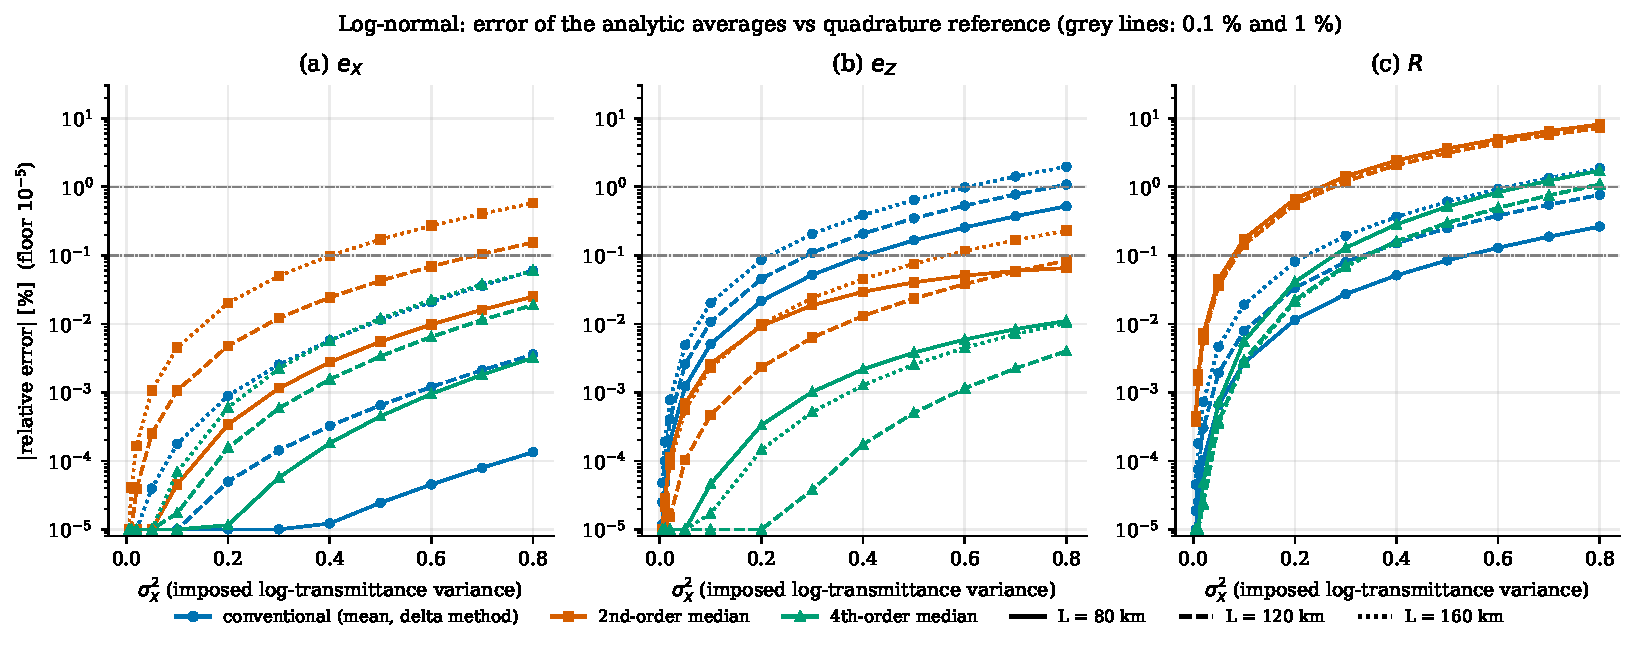
\includegraphics[width=\linewidth]{sens_fig_LN.pdf}\caption{Log-normal channel.}\label{fig:LN}\end{figure}
\begin{figure}[htbp]\centering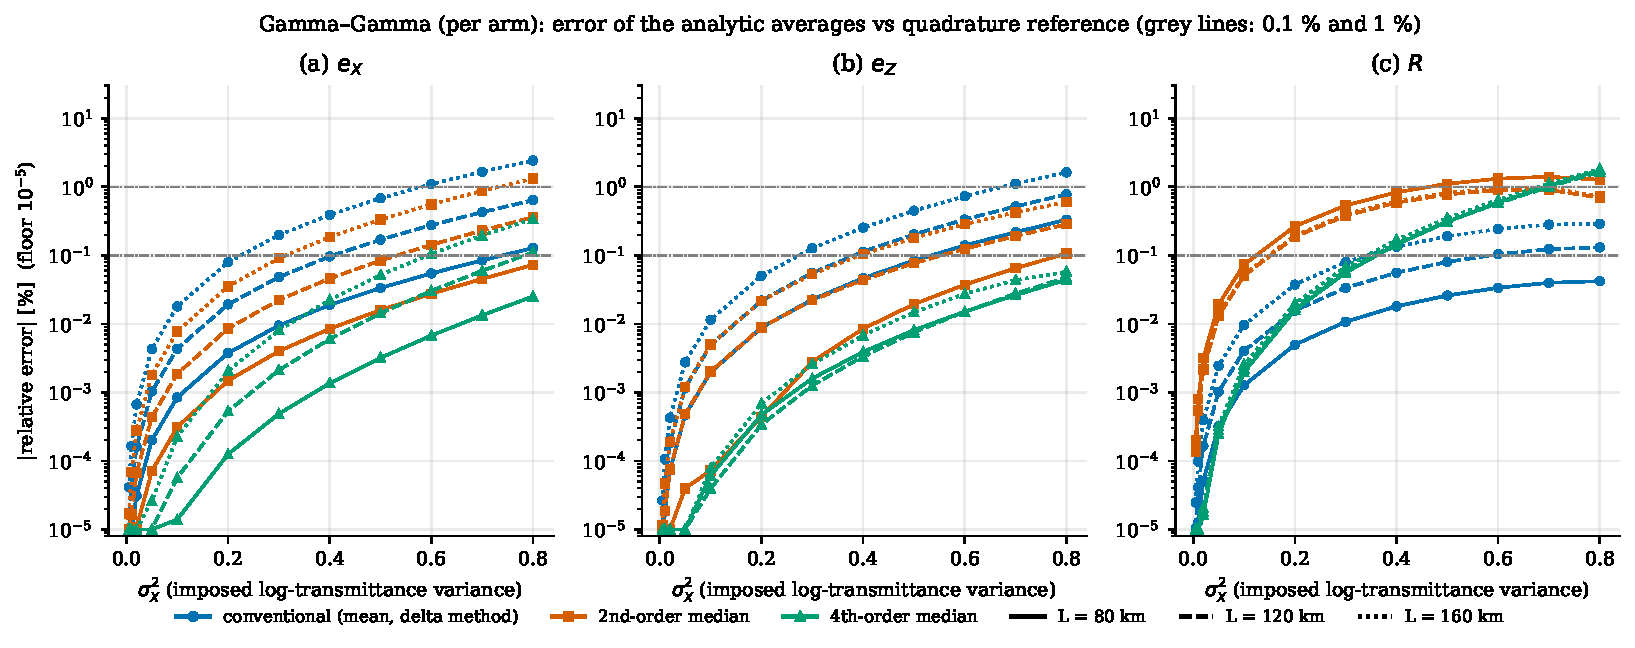
\includegraphics[width=\linewidth]{sens_fig_GG.pdf}\caption{Gamma--Gamma channel (per arm).}\label{fig:GG}\end{figure}
\begin{figure}[htbp]\centering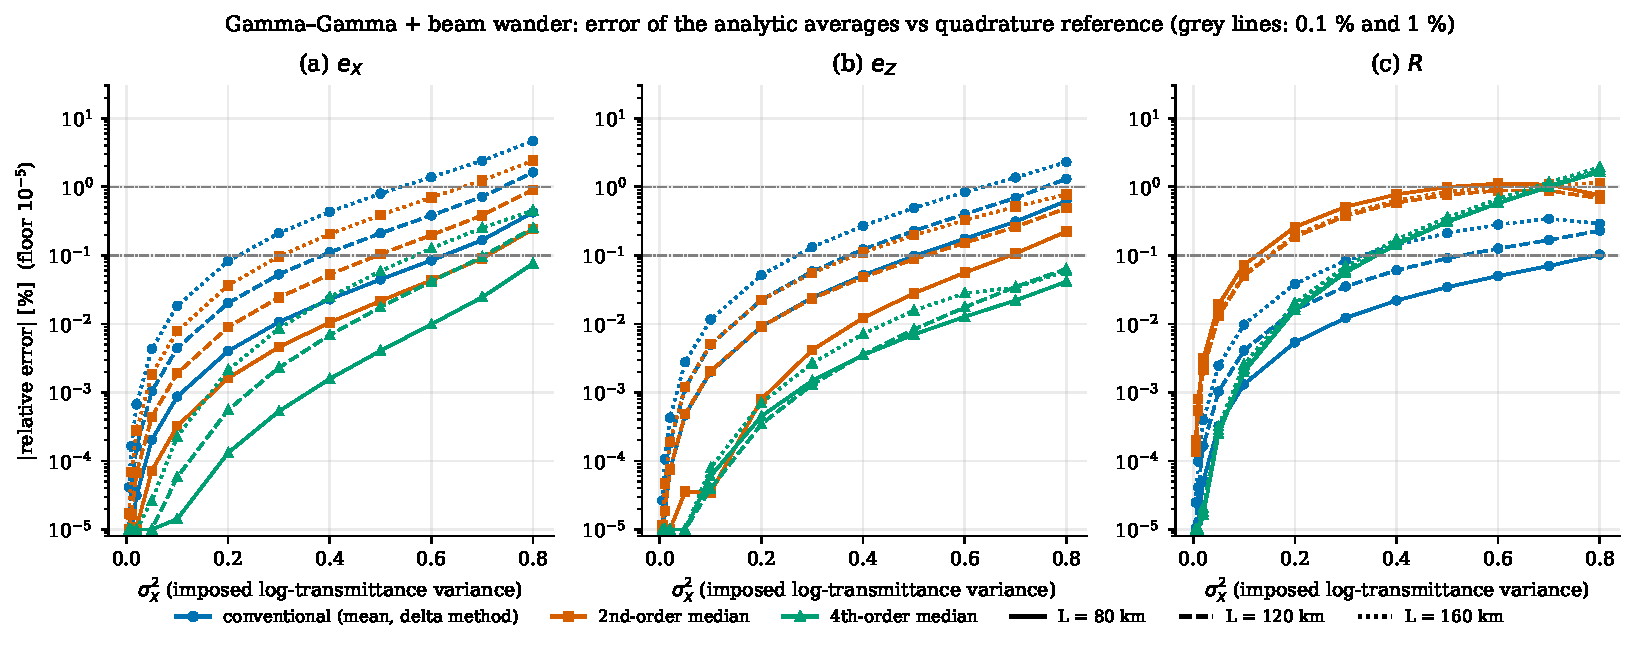
\includegraphics[width=\linewidth]{sens_fig_GGBB.pdf}\caption{Gamma--Gamma channel with beam wander (long-term beam broadening).}\label{fig:GGBB}\end{figure}

\section{Answers established by the data}
\paragraph{1. Does the approximation error increase with turbulence strength?}
Yes, in general. Of the $81$ (model, $L$, quantity, approximation) curves, $72$ increase monotonically in $|{\rm error}|$ over the grid and $9$ do not. The exceptions are the 2nd-order key-rate error of GG and GG+BB at all three distances (six curves; $|{\rm error}|$ peaks at $\sigma_X^2\approx0.6$--$0.7$ and then falls slightly, $1.40\to1.26\%$ at $80$~km for GG), the 2nd-order $e_Z$ of GG at $80$~km, and two small non-monotonicities at GG+BB, $160$~km (mean-approximation $R$, 4th-order $e_Z$). The size and the ranking of the errors depend on the quantity and on the distance (Table~\ref{tab:thr}, \ref{tab:thr2}): errors grow with distance at fixed $\sigma_X^2$ for $e_X$ and $e_Z$ in the GG models (e.g.\ mean-approximation $e_X$ error at $\sigma_X^2=0.8$: $0.13\%$, $0.64\%$, $2.4\%$ at $80,120,160$~km), because the operating point moves to a smaller $\eta_0$ where the error rates vary faster in $\ln\eta$. For $R$ the 4th-order error at $\sigma_X^2=0.8$ is nearly distance independent ($1.6$--$1.9\%$ in GG, $1.1$--$1.7\%$ in LN).

\paragraph{2. When does the 2nd-order approximation become insufficient for the key rate?}
Taking $0.1\%$ as the threshold for a ``precise'' value and $1\%$ for a ``usable'' one: the 2nd-order key-rate error exceeds $0.1\%$ at $\sigma_X^2\approx0.08$--$0.09$ for the log-normal channel and at $0.125$--$0.153$ for Gamma--Gamma, with or without beam wander; it exceeds $1\%$ at $\sigma_X^2\approx0.25$--$0.28$ (LN, all distances) and $0.47$ ($80$~km, GG), $0.51$ (GG+BB, $80$~km), and $0.65$ (GG+BB, $160$~km); for GG at $120$ and $160$~km and GG+BB at $120$~km it stays below $1\%$ up to $0.8$ (maxima $0.89$, $0.93$, $0.87\%$). The log-normal 2nd-order error reaches $7$--$8\%$ at $\sigma_X^2=0.8$. Conclusion: for the key rate the 2nd-order formula stops being accurate (to $0.1\%$) at $\sigma_X^2\approx0.1$, and (to $1\%$) at $\approx0.25$ in log-normal and around $0.5$ or not within the grid in Gamma--Gamma. At the realistic weak-class points ($\sigma_X^2=0.086$--$0.307$ LN, $c_2=0.084$--$0.258$ GG) the 2nd-order key-rate error, interpolated on the grid, is about $0.06$, $0.14$, $0.3\%$ (GG, $80,120,160$~km) and $0.13$, $0.5$, $1.3\%$ (LN).

\paragraph{3. Does the 4th-order approximation stay accurate over the tested range?}
It depends on the quantity.
\begin{itemize}
\item \emph{$e_X$ and $e_Z$:} yes. The 4th-order error stays below $0.46\%$ everywhere and below $0.1\%$ for all LN cases and for GG at $80$~km; its maximum is $0.45\%$ ($e_X$, GG+BB, $160$~km) and $0.06\%$ for $e_Z$. At $\sigma_X^2=0.8$ it is the best of the three approximations for $e_Z$ in every case and for $e_X$ in all GG and GG+BB cases and in LN at $160$~km (in LN at $80$ and $120$~km the mean approximation is marginally better for $e_X$, $\le0.004\%$).
\item \emph{$R$:} the error is bounded ($\le1.9\%$ for $\sigma_X^2\le0.8$) but it is \emph{not} uniformly small. It exceeds $0.1\%$ at $\sigma_X^2\approx0.28$--$0.36$ (LN $0.28$--$0.35$, GG and GG+BB $0.34$--$0.36$) and $1\%$ at $\approx0.65$--$0.78$ (LN $0.65$ at $80$~km and $0.78$ at $120$ and $160$~km; GG and GG+BB $0.68$--$0.70$). In Gamma--Gamma the 4th-order error \emph{overtakes} the 2nd-order one at $\sigma_X^2\approx0.7$ ($L=120,160$~km) and $0.8$ ($80$~km, GG and GG+BB): adding the $\Theta^3,\Theta^4$ terms no longer improves the result, i.e.\ the cumulant series is asymptotic and the third and fourth cumulants are no longer small corrections there. In the log-normal channel the 4th order is better than the 2nd throughout ($1.1$--$1.7\%$ against $7$--$8\%$ at $0.8$).
\item \emph{Surprise in the data:} the conventional mean-transmittance approximation is the \emph{most} accurate for $R$ at $\sigma_X^2=0.8$ in all GG and GG+BB cases ($\le0.30\%$) and in LN at $80$--$120$~km, although it is the worst for $e_X$ and $e_Z$. This is not evidence of a controlled expansion: at these operating points $R(\eta)$ is locally close to a power law ($d\ln R/d\ln\eta=1.05$--$1.13$ at $80$--$160$~km in the repository), for which the curvature correction in $\eta$ is small, and the delta-method error at $160$~km in the log-normal model already grows to $1.7\%$ at $\sigma_X^2=0.8$.
\end{itemize}

\paragraph{Beam wander.} In this controlled setting beam wander only shifts $\eta_0$ by $f_{\rm bb}$ (from $0.999$ to $0.09$--$0.18$ at $\sigma_X^2=0.8$); the key rate itself drops by up to a factor $3.6$ ($2.8$--$3.6$ at $\sigma_X^2=0.8$). The relative errors of $R$ differ from the plain GG case by at most $0.13$ percentage points. The errors of $e_X$ and $e_Z$ grow with the shift towards smaller $\eta_0$, mostly at $160$~km (mean approximation $e_X$ at $\sigma_X^2=0.8$: $2.4\to4.7\%$; 4th order: $0.34\to0.45\%$). The analytic formulas therefore keep their accuracy for the key rate with the beam-wander loss, and lose some for $e_X$ with the conventional approximation, \emph{provided} the shifted operating point stays on the smooth branch of the key-rate curve (all $\eta_m$ here do; $R(\eta_m)\ge6\times10^{-6}$).

\section{Limits}
Only $\sigma_X^2\le0.8$ was tested (the Gamma--Gamma maximum is $0.858$); log-normal behaviour above that, where the repository's validity limit $\sigma_R^2=1$ ($\sigma_X^2=0.5$) is already exceeded for $\sigma_X^2>0.5$, is not covered. The imposed values at fixed distance are a sensitivity device. Error values below $10^{-5}\%$ are plotted at a floor. Reproduction: \texttt{paper\_analysis/scripts/sensitivity\_study.py}, \texttt{sensitivity\_thresholds.py}, \texttt{sensitivity\_figures.py}, \texttt{sensitivity\_make\_tex.py} (they import the repository unchanged).
\end{document}
